%!TEX root = ../thesis.tex

\subsection{Sweepcycle algorithm}
\thispagestyle{plain}
  \label{ss:sweep}
  \fxnote{Note the lack of proof?}
  The first step of our algorithm is executing a sweepcycle algorithm inspired by Fusy's \cite{Fusy2006}. We use $\C$ to indicate the current sweep cycle.



  %

  %Then $p_1$ and $p_k$ indicate the two unique vertices of the walk that are also part of the cycle. We will then let $\restC{\P}$ denote the part of $\cpath$ that is between $p_1$ and $p_k$ (including). $\C_\P$ will denote the cycle given by $\restC{\P} \oplus \rev{\P}$.

  During the algorithm we will want to maintain several invariants on $\C$. The first three are equivalent to those imposed by Fusy. The final invariant is new and imposes a nice structure on the sweepcycle so far. \fxnote{Can i be more precise}

  \begin{invariants}
    \itemsep=-4pt

    \item \label{i:uni:SWandSE} The cycle $\C$ contains the two edges $\pS \pW$ and $\pS \pE$.
    \item \label{i:uni:noChords} $\cpath$ has no chords
    \item \label{i:uni:intVertCond} All inner edges of $G$ in the exterior of $\C$ are colored and oriented such that the inner vertex condition holds for all vertices in the exterior of $C$.
    \item \label{i:uni:no2Chords} $\C\sm{\pS}$ has no separating 2-chords that do not use $\S$
  \end{invariants}

  We denote the vertices of the sweepcycle $\C$ by $\pS, v_1 = \pW, v_2, \ldots v_{n-1}, v_n = \pE, \pS$.   We will repeatedly consider the path $\cpath$. In that case we will always order it from $\pW$ to $\pE$. That these edges are always in $\C$ is a result of Invariant \ref{i:uni:SWandSE}.


  Each update of the sweepcycle consists of the following three steps
  \begin{enumerate}
    \itemsep=-4pt
    \item Take the right neighbor walk of a suitable subpath of $\cpath$ to obtain the \emph{candidate path} $P$.
    \item Evade chords and separating $2$-chords on $P$ to obtain the \emph{updating path} $P'$.
    \item Update the sweepcycle with $P'$.
  \end{enumerate}

  We repeat these steps until the sweepcycle does not contain any more interior vertices. At which point we can terminate the algorithm by coloring the edges still on the cycle $\C$ blue and its interior edges red.

  \subsubsection{Find the right neighbor path}
    Let $v_i$ denote all the vertices of $\cpath$ in the following order $\pW =  v_1   v_2   \ldots v_{n-1}   v_n = \pE$.
    Some intervals of these vertices will be adjacent to $\pS$. However, they can not be all adjacent to $S$ since then any vertex still in the interior of $\C$ would lie in a separating triangle of $G$. So we have no interior vertices and hence we can terminate the algorithm as described in Section \ref{sss:terminating}. We denote by $v_i$ the last vertex of first interval of vertices adjacent to $S$ and by $v_j$ the first vertex of the second interval.
    As candidate path $P$ we take the right neighbor path of $\cpath|_{v_i, v_j}$. This right neighbor path does indeed exist since all interior vertices of $\cpath|_{v_i, v_j}$ are interior vertices of $G$ and $\cpath$ has no cycles or separating 2-chords by Invariants \ref{i:uni:noChords} and \ref{i:uni:no2Chords}.
    The current situation is also depicted in Figure \ref{fig:sweep:rightNeighbourwalk}.

    \begin{figure}[h]
      \centering
      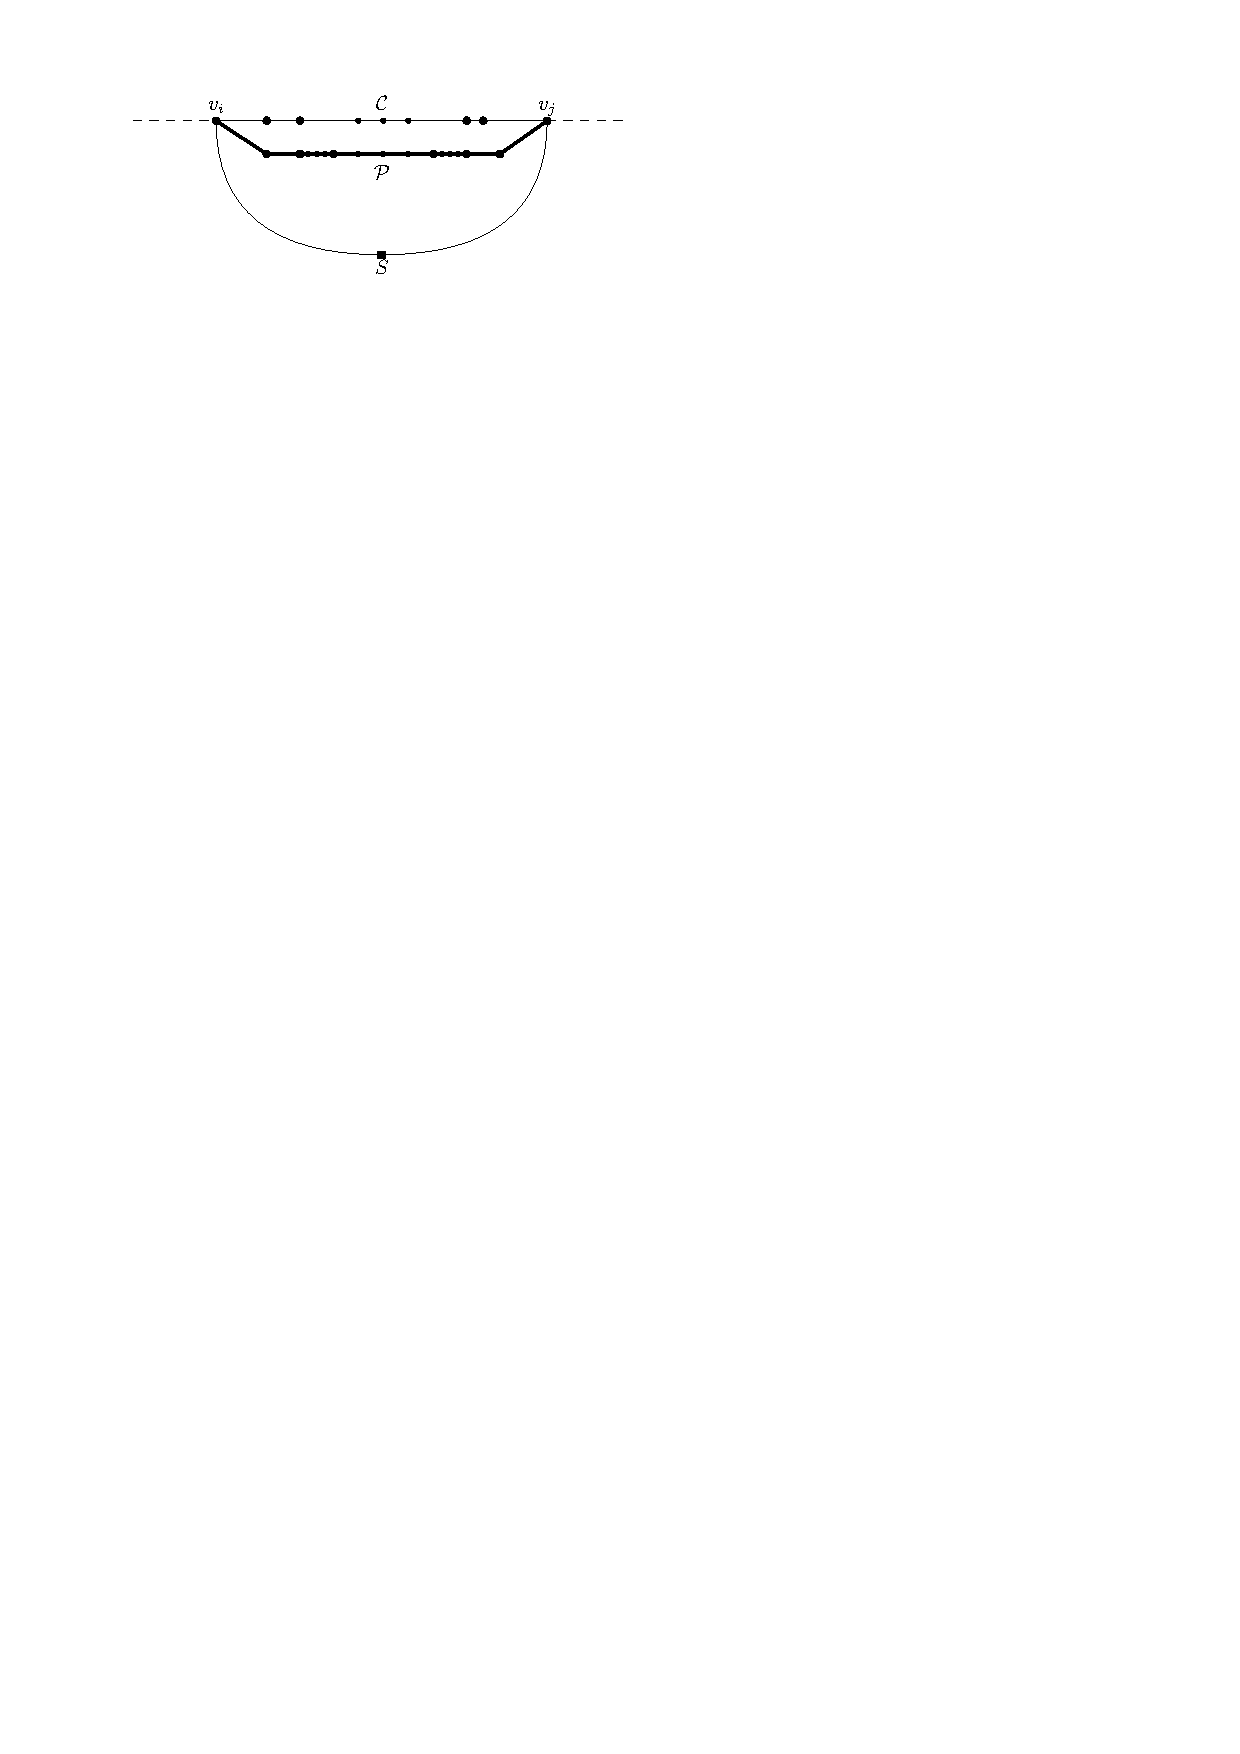
\includegraphics[scale=1]{unifiedAlgo/img/sweep/rightNeighbourWalk}
      \caption{}
      \label{fig:sweep:rightNeighbourwalk}
    \end{figure}

  \subsubsection{Irregularities}
    The candidate path $P$ we found can have several structures we want to avoid
    namely
    \begin{enumerate}
      \itemsep=-4pt
      \item Chords
      \item Separating 2-chords
    \end{enumerate}

    Both of these structures are on the right of the candidate path due to Lemma \ref{lm:right:neighbourwalkChordFree} (no chords on the left) and Lemma \ref{lm:right:neighbourwalkNoInteriorVertex} (no separating 2-chords on the left).

    To evade these structures we firs have to introduce more notation. We orient $P$ from $v_i$ (the vertex closest to $\pW$)to $v_j$ (the vertex closest to $\pE$) and denote its vertices by $p_1 \ldots p_k$. The \emph{index} of a vertex $p_i \in P$ is its position in the path, that is, the index of $p_i$ is $i$.

    The \emph{range} of an irregularity will be given by its start and end index. Depending on what irregularities we find on the candidate path we will update the sweepcycle with a \emph{update path} $P'$. This update is described in \ref{sss:sweep:update}.

    \mypar{We have no irregularity}
      When there are no irregularities we update the sweepcycle with the entire candidate path $\P$. The update path $P'$ is $P$ in this case.

    \mypar{We have any chord}
    We know that we can not have any polebound chords on the candidate path since any such chord would offend Invariant \ref{i:uni:no2Chords} of the sweepcycle.
    \fxwarning{Show this polebound thing using a figure}

    If our candidate path has any chords we look identify the them by their start and end vertex. Of the chords with the lowest start index we will consider the one with the largest end index. We denote this chord by $C_\text{outer}$.

    We now consider $C_\text{outer}$ and any chord contained therein. In this collection we look for the chord $C_\text{inner}$ with the smallest range (i.e. highest start $i$ and lowest end $j$).
    The way in which these chords are chosen is illustrated in Figure \ref{fig:sweep:chordsOnCandidatePath}.

    \begin{figure}[b]
      \centering
      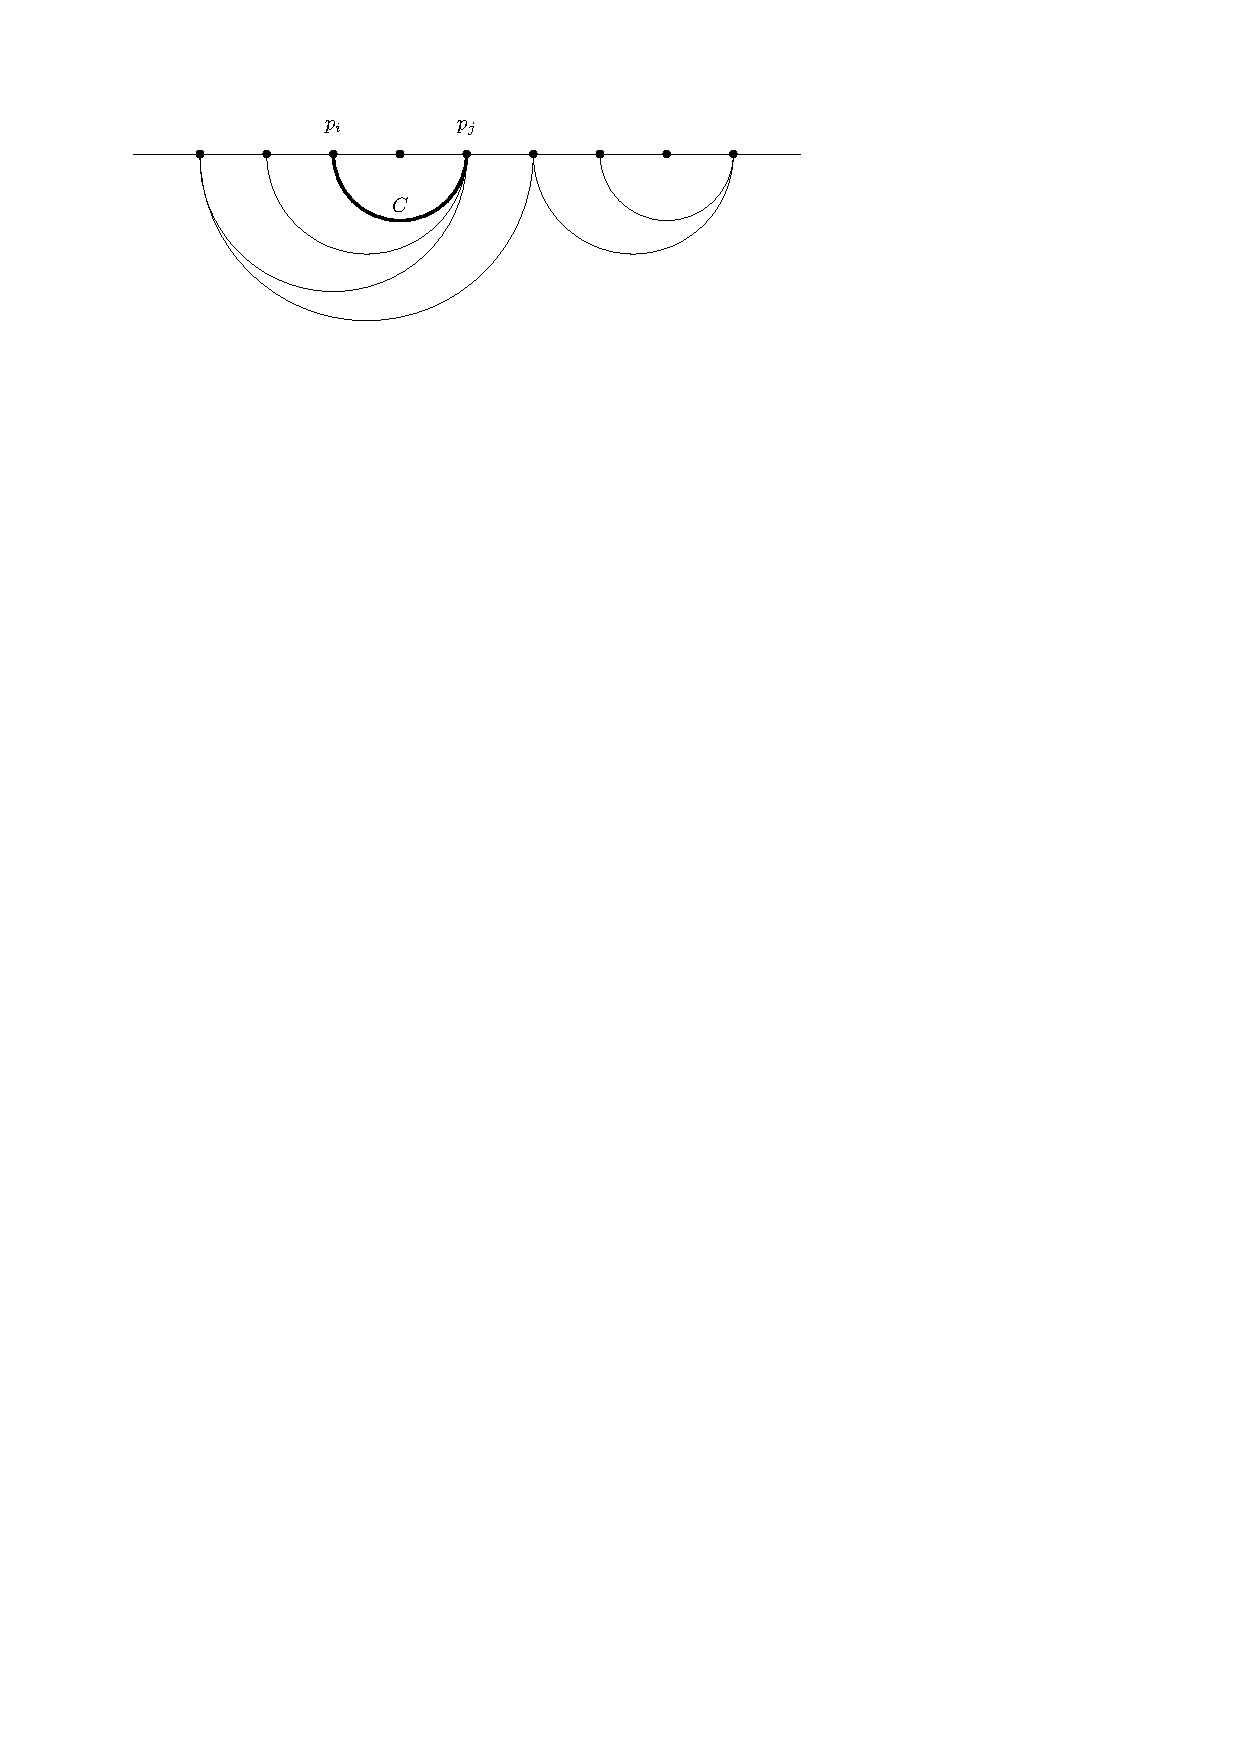
\includegraphics[scale=1]{unifiedalgo/img/sweep/chordsOnCandidatePath}
      \caption{}
      \label{fig:sweep:chordsOnCandidatePath}
    \end{figure}

    What we do now depends on whether a 2-chord shows up in the interior of the chord pasted to the candidate path $\P|_{i, j} \oplus \rev{{C_\text{inner}}}$.

    \emph{No separating 2-chord.}
    If there is no separating 2-chord in the interior of $\P|_{i, j} \oplus \rev{{C_\text{inner}}}$ we do the following. Let $v_k$ be the shared neighbor on the sweepcycle of $p_{i}$ $p_{i +1}$ and $v_l$ the shared neighbor on the sweepcycle  of $p_{j -1}$ and $p_{j}$. Then the updating path is the right neighbor path of $\cpath|_{v_k, v_l}$. See Figure \ref{fig:sweep:chordUpdate}.

    \begin{figure}[h]
      \centering
      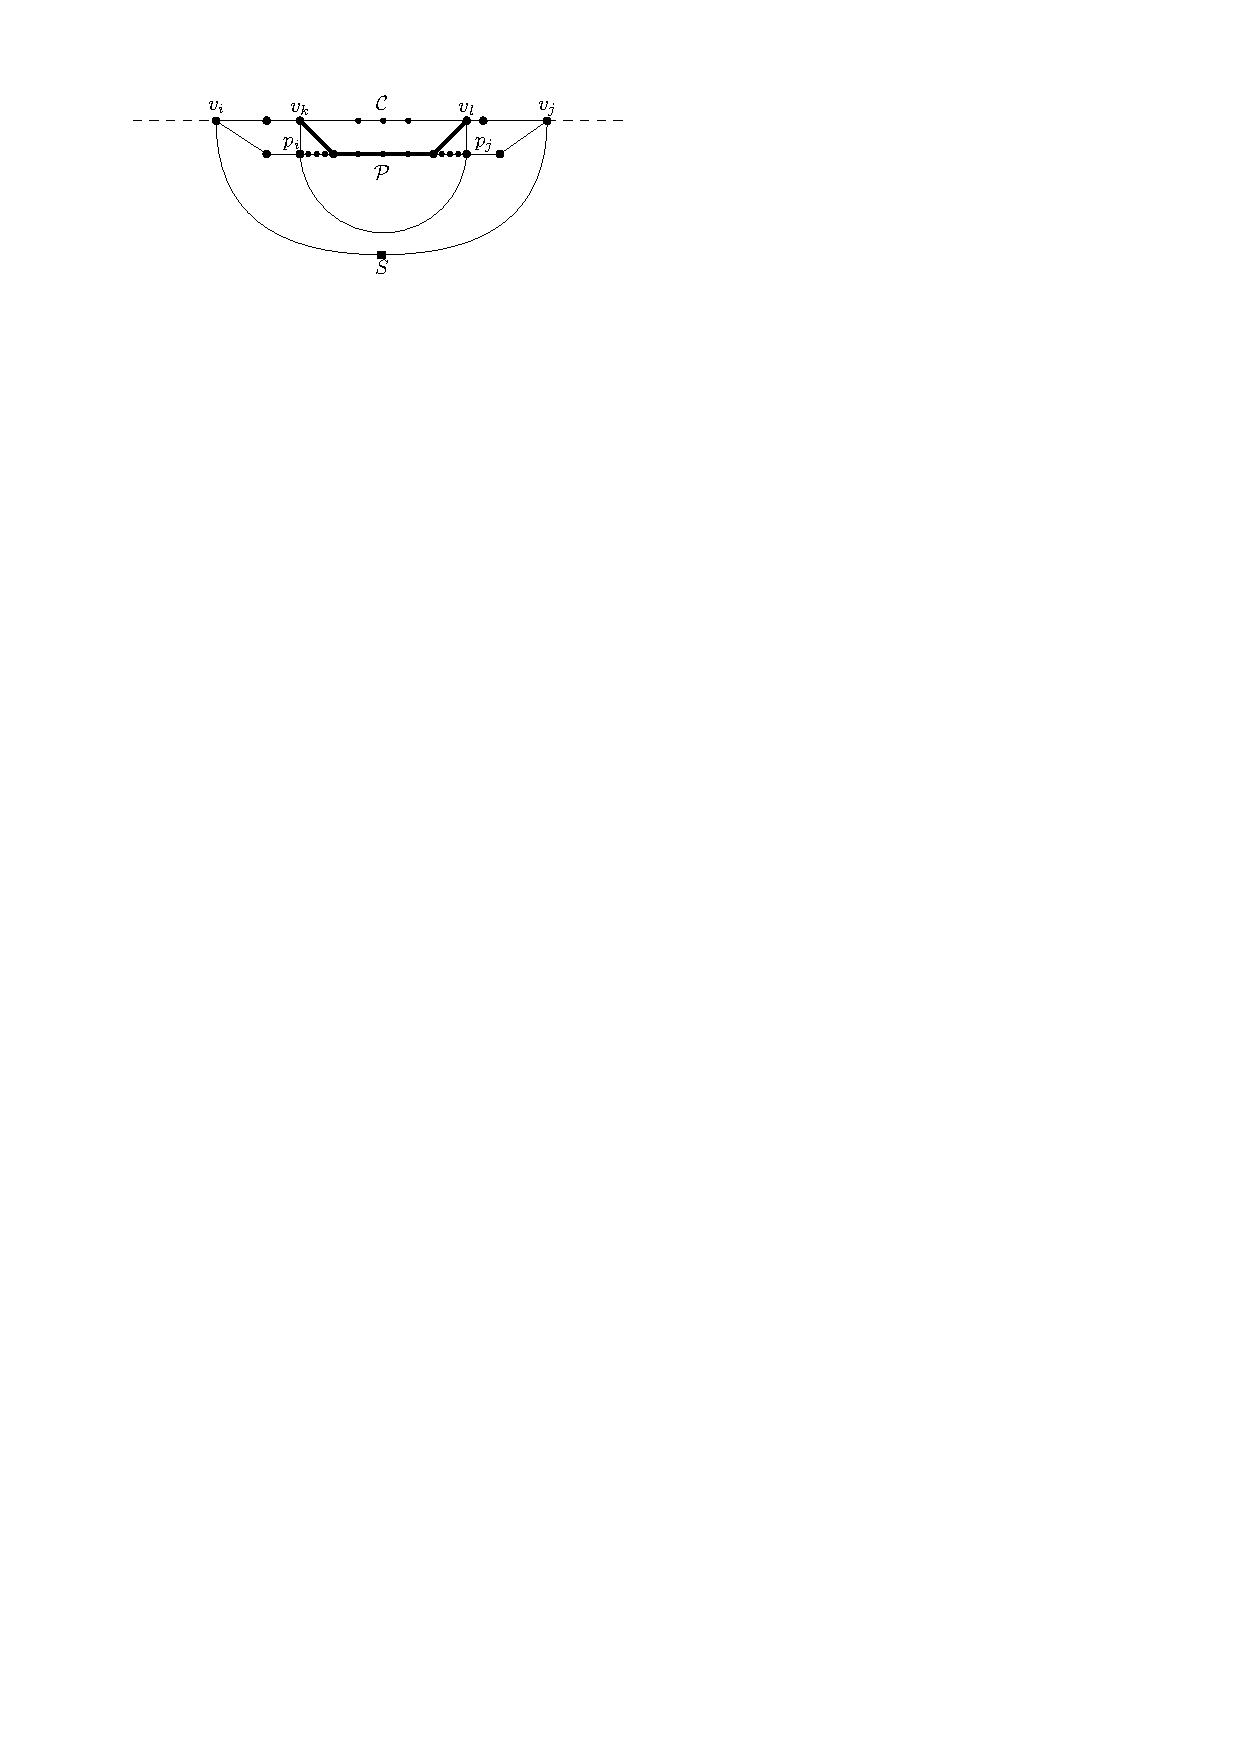
\includegraphics[scale=1]{unifiedAlgo/img/sweep/chordUpdate}
      \caption{}
      \label{fig:sweep:chordUpdate}
    \end{figure}

    \emph{At least one separating 2-chord.}
      \fxinnote{None of these are polebound. Be more clear when indicating what an end range is}
      Let $j'$ be end index of the separating 2-chord with the lowest end range in the interior of $\P|_{i, j} \oplus \rev{{C_\text{inner}}}$. And let $v_k$ be the shared neighbor on the sweepcycle of $p_{i_1}$ $p_{i_1 +1}$ and $v_l$ the shared neighbor on the sweepcycle  of $p_{j' -1}$ and $p_{j'}$.
      Then the updating path is the  right neighbor path of $\cpath|_{v_k, v_l}$. See Figure \ref{fig:sweep:2chordInChordUpdate}.

    \begin{figure}[h]
      \centering
      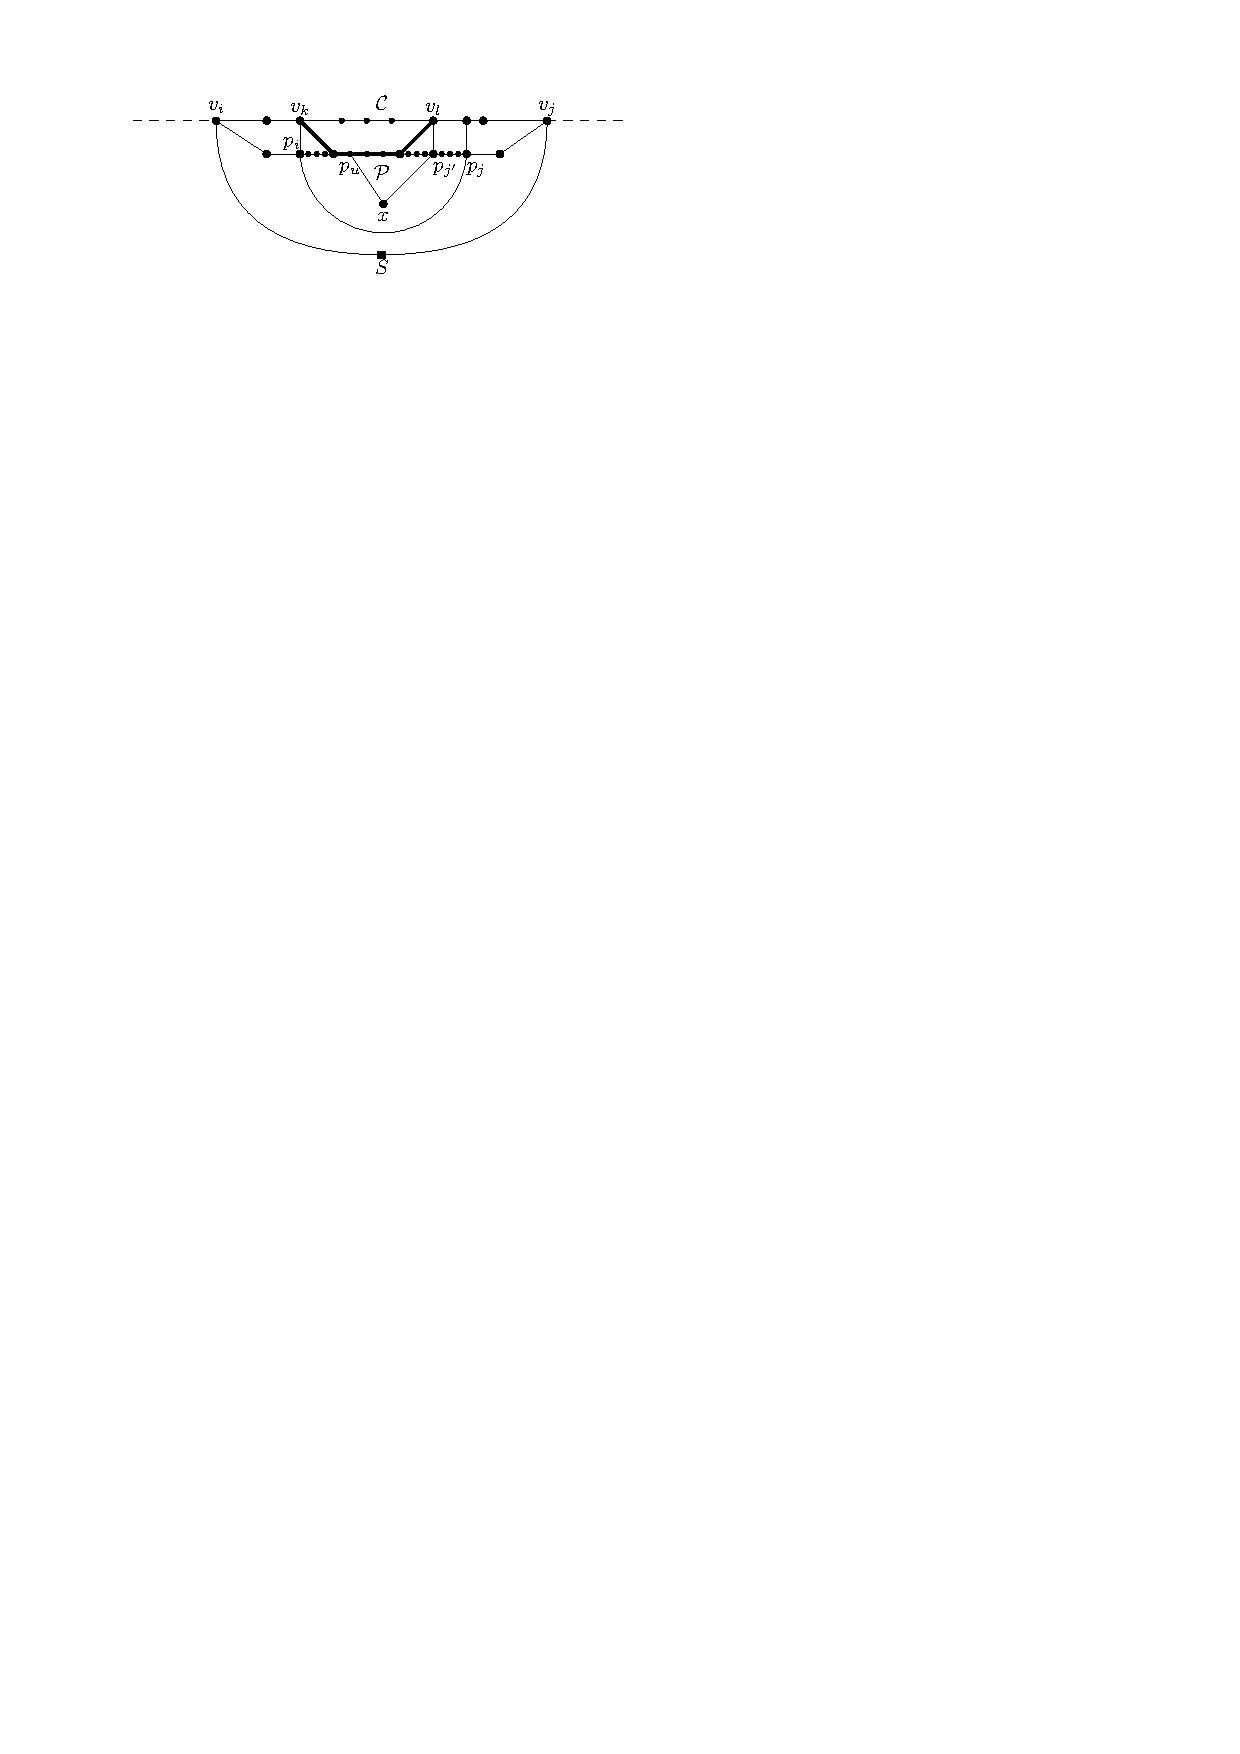
\includegraphics[scale=1]{unifiedAlgo/img/sweep/2chordInChordUpdate}
      \caption{}
      \label{fig:sweep:2chordInChordUpdate}
    \end{figure}

    \mypar{Only separating 2-chords}
    \emph{Any $\pE$-bound 2-chords}
    Start a path inside the smallest 2-chord (i.e. with the highest starting number for its range). Say the start of this range is $i$ we then update the sweepcycle in the following way.

    Let $v_k$ be the shared neighbor on the sweepcycle of $p_{i}$ $p_{i +1}$. The updating path is the right neighbor path of $\cpath|_{v_k, \pE}$. See Figure \ref{fig:sweep:pEBound}.

    \begin{figure}[h]
      \centering
      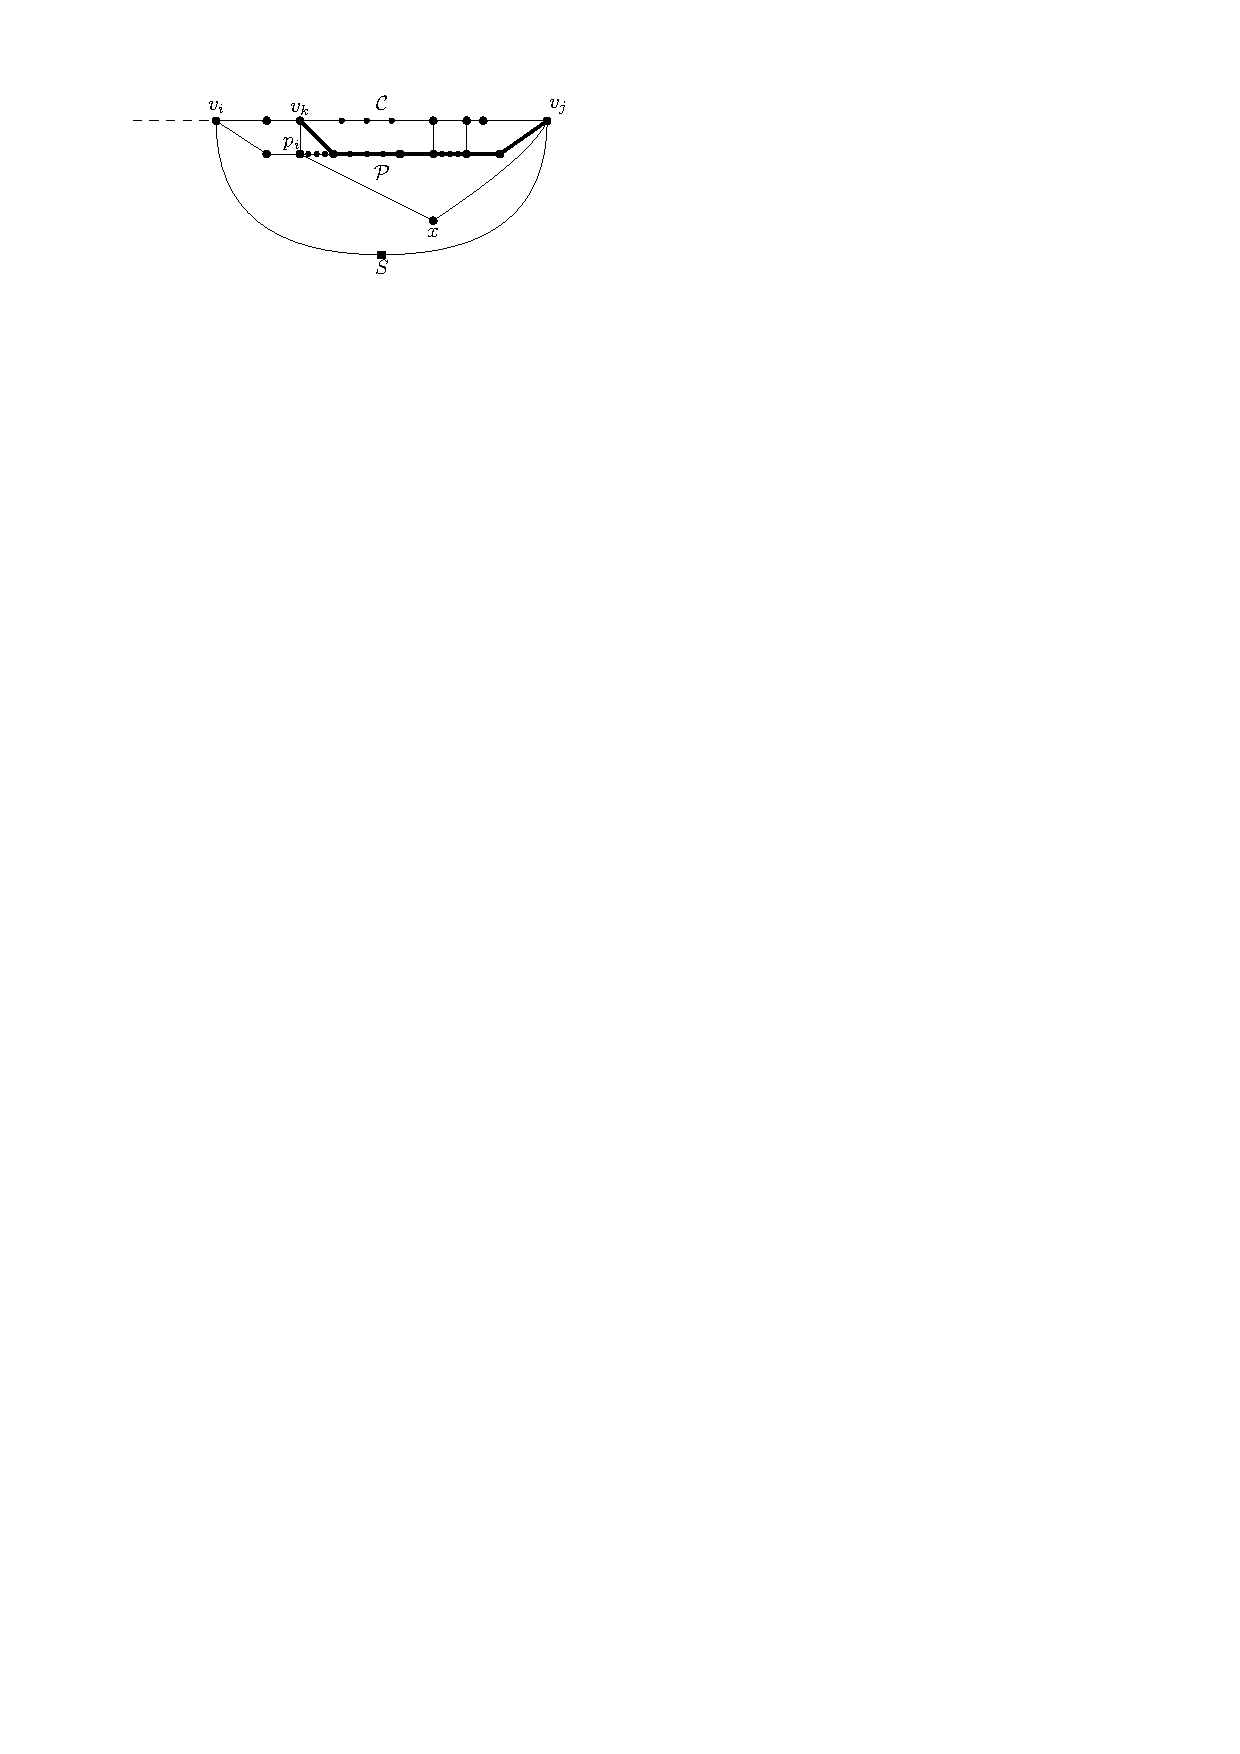
\includegraphics[scale=1]{unifiedAlgo/img/sweep/pEBound}
      \caption{}
      \label{fig:sweep:pEBound}
    \end{figure}
    \emph{Other separating 2-chords}
    The 2-chord can not contain a chord since then we would be in the above case.
    Find the $2$-chord with the lowest end of range. Say that this is $j$. We then update the sweepcycle in the following way.

    Let $v_l$ be the shared neighbor on the sweepcycle of $p_{j}$ $p_{j-1}$. The updating path is the right neighbor path of $\cpath|_{v_i, v_l}$. See Figure \ref{fig:sweep:free2chord}.

    \begin{figure}[b]
      \centering
      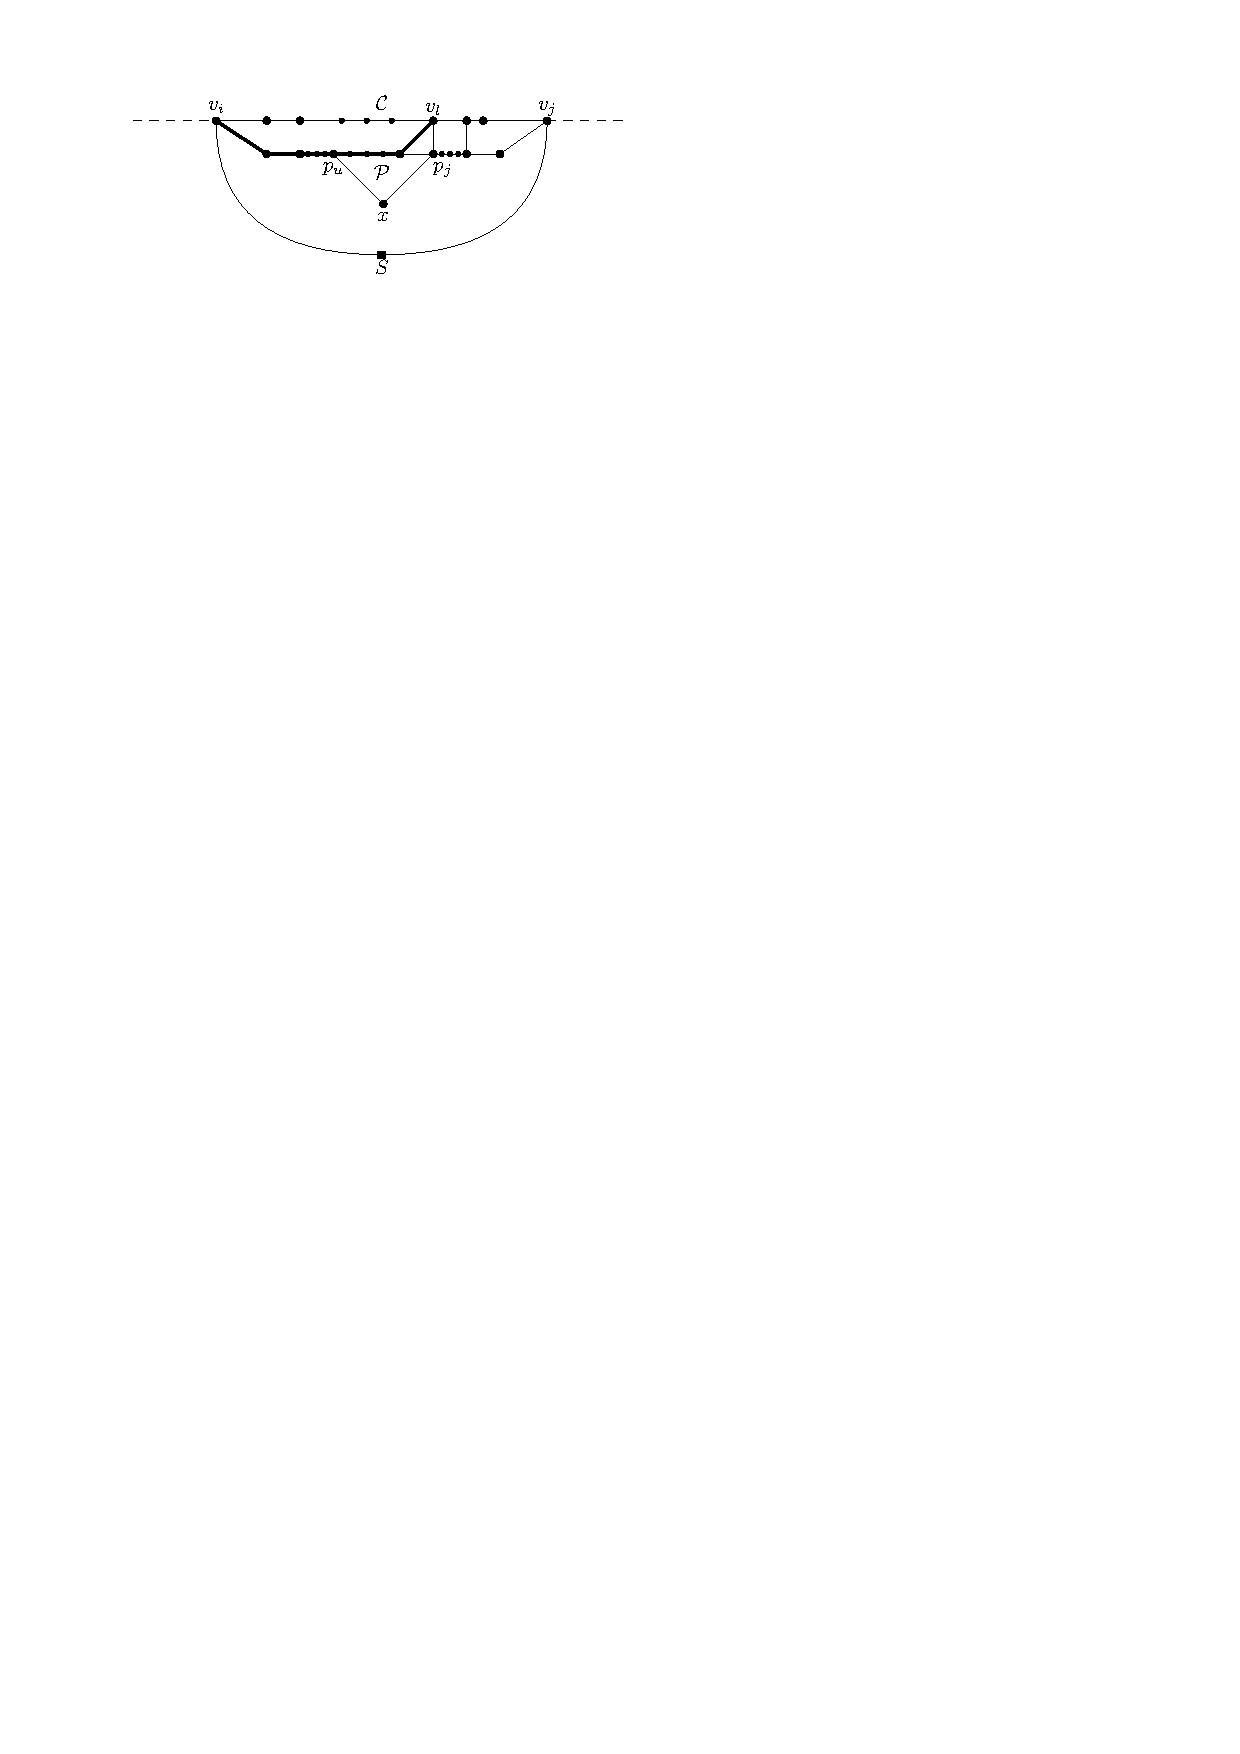
\includegraphics[scale=1]{unifiedAlgo/img/sweep/free2chord}
      \caption{}
      \label{fig:sweep:free2chord}
    \end{figure}

  \subsubsection{Updating}
    \label{sss:sweep:update}
    Once we found the updating path $P'$ we can update the sweepcycle with this path. Here we describe how we do this we also show that the update maintains the sweepcycle invariants \ref{lm:sweep:updateMaintainsInvariants}. We first color all interior edge of $\cpath|_{P'} \oplus \rev{P'}$ red and orient them towards $\cpath|_{P'}$. We also color all edges of $\cpath|_{P'}$  blue and orient them from lower to higher induces. We then update the sweepcycle to $\C'$ by replacing $\cpath|_{v_i,v_j}$ by $P'$.


    \begin{lemma}
      The updating paths have no chords or separating $2$-chords
      \label{lm:sweep:augNoIregularity}
    \end{lemma}
    \begin{proof}
        All of these structures are on the right of the updating path, since the updating path is a subset of a right neighbor path and a right neighbor path satisfies Lemma \ref{lm:right:neighbourwalkChordFree} (no chords on the left) and Lemma \ref{lm:right:neighbourwalkNoInteriorVertex} (no separating 2-chords on the left).

        If the candidate path had any chords the updating path is adapted to be entirely inside a chord containing no more chords. Hence the updating path can not have any chords.

        Moreover any updating path stops before the end of a separating 2-chord unless it is a $\pE$-bound separating 2-chord in which case it only starts after the begin of this 2-chord. Either way the updating path also has no separating 2-chords.
    \end{proof}

    \begin{lemma}
      \label{lm:sweep:noConnectingIregularity}
      There are no chords or separating $2$-chords not containing $\pS$ with one endpoint on the old sweepcycle and the other endpoint on the updating path.
    \end{lemma}

    \begin{proof}
      \emph{No irregularity}
      Since $v_i$ and $v_j$ are both adjacent to $\pS$ we can not have any chords. And any $2$-chords have $\pS$ as middle vertex. However these are allowed for the Lemma.

      \emph{Chord, not containing a 2-chord}
      Any chord or separating $2$-chord will have to cross $v_k p_i p_j v_l$ so we can not have a chord. Any 2-chord has to have $p_i$ or $p_j$ as middle vertex. But with this restriction the 2-chord can not be separating.

      \emph{Chord, containing a 2-chord}
      In the same manner as in the above case we can not expect any chord or separating 2-chord to connect outside the containing chord.
      Suppose that we have a separating $2$-chord then that would have been a chord of the candidate path. This is in contradiction with the fact that the outer chord contained no more chords.
      Suppose that we have a chord not connecting to the second-to-last vertex of the updating path. This chord would offend Invariant \ref{i:uni:no2Chords} of the old sweepcycle. Furthermore the second-to-last vertex of the updating path has no chords since it would break $v_l p_j x p_u$. (see Figure \ref{fig:sweep:2chordInChordUpdate}).

      \emph{$\pE$-bound separating $2$-chord}
      We can not have any chords since these would have to break $\pE x p_i v_k$. Any $2-chords$ would have $x$ or $p_i$ as middle vertex. However the first yields a $2$-chord of the candidate path with a higher start range, this is a contradiction. And the second can not yield an separating $2$-chord.


      \emph{Other separating $2$-chord}
      Any chord or $2$-chord with one vertex in the updating path and the other on the old sweepcycle must end to the right of the updating path since the updating path starts at $\pW$.
      Suppose that we have a separating $2$-chord then that would have been a chord of the candidate path. This is in contradiction with the assumption that the candidate path had no chords.
      Suppose that we have a chord not connecting to the second-to-last vertex of the updating path. This chord would offend Invariant \ref{i:uni:no2Chords} of the old sweepcycle. Furthermore the second-to-last vertex of the updating path has no chords since it would break $v_l p_j x p_u$. (see Figure \ref{fig:sweep:free2chord}).
    \end{proof}

    \begin{lemma}
      \ref{lm:sweep:updateMaintainsInvariants}
      All five updating path types maintain the sweepcycle invariants
    \end{lemma}
    \begin{proof}
      We will proof that the new sweepcycle $\C'$ obtained by updating $\C$ is again a valid sweepcycle. Invariant \ref{i:uni:SWandSE} remains trivially true. Invariant \ref{i:uni:intVertCond} hold due to the way we colored the edges around the new interior vertices.

      To see that Invariants \ref{i:uni:noChords} and \ref{i:uni:no2Chords} hold note that there can be no chords or $2$-chords with both endpoints in the overlap of the old and new sweepcycle $\C \cap \C'$ by the same Invariants \ref{i:uni:noChords} and \ref{i:uni:no2Chords}. Since the updating path itself also has no irregularities (Lemma \ref{lm:sweep:augNoIregularity}),
      we know any chord or separating $2$-chord $C$ has to have one vertex on $\P$ and one vertex on the unchanged part of old sweepcycle $\C \cap \C'$. However these potential chords are also not offending by Lemma \ref{lm:sweep:noConnectingIregularity}.

      Hence $\C'$ is a valid new sweepcycle.
    \end{proof}

    If after the update the new sweepcyle $\C'$ is not separating we do not do another update round and we instead terminate the algorithm as will be described in Section \ref{sss:terminating}.

  \subsubsection{Terminating}
    \label{sss:terminating}
    When the sweepcycle is no longer separating we can not update it anymore. However at this point it is easy to color the remainder of the graph. All vertices in $\C$ must be adjacent to $\pS$ since $\pS \pW$ and $\pS \pE$ are part of $C$ by Invariant \ref{i:uni:SWandSE} $C$ has no chords by Invariant \ref{i:uni:noChords} and $C$ does not contain any interior vertices. Since all vertices are adjacent to $\S$ all sweepcycle interior edges are adjacent to $\pS$.

    We color all interior edges of $\C$ red and orient them towards $\cpath$ and the edges in $\cpath$ are colored blue and oriented towards $\pE$. This last move completes the interior vertex condition for vertices in $\C \sm {\pW, \pS, \pE}$ and also correctly completes the exterior vertices.


    \begin{lemma}
      \label{lm:sweep:REL}
      The resulting structure is a REL
    \end{lemma}

    \begin{proof}
      After running the whole algorithm the interior vertex condition holds for all vertices in the graph. Furthermore the poles are also colored correctly due to Invariant \ref{i:uni:SWandSE}.
    \end{proof}

    Given a splitvertex $v$ we will by \emph{bottom} path mean the path that comes in trough the first incoming blue edge in the the rotation at $v$ and leaves through the last outgoing blue edge in the rotation at $v$. See Figure \ref{fig:sweep:bottomPath}.

    \begin{figure}[h]
      \centering
      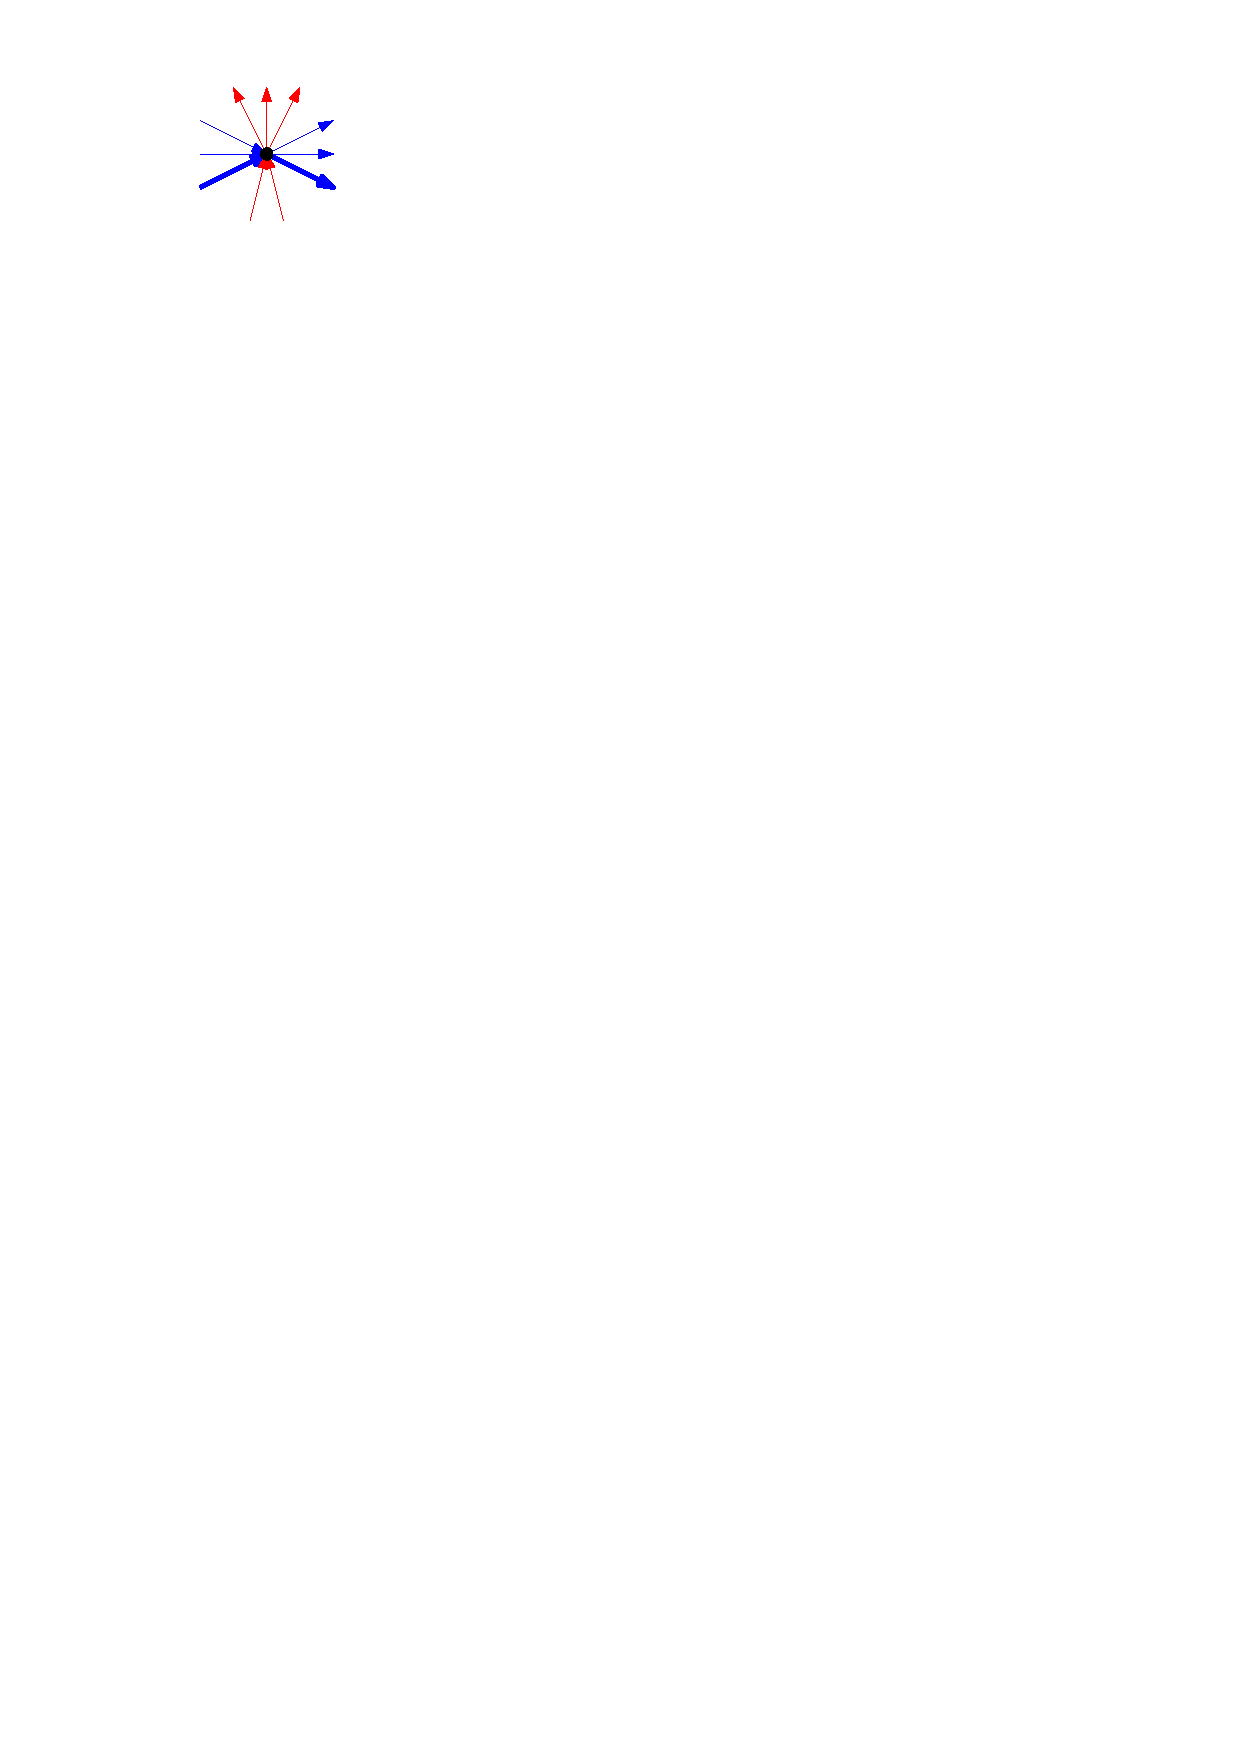
\includegraphics[scale=1]{unifiedAlgo/img/sweep/bottompath.pdf}
      \caption{The bottom path of this splitvertex is given in bold}
      \label{fig:sweep:bottomPath}
    \end{figure}

    \begin{lemma}
      \label{lm:sweep:NoTwoSplitsAboveEachOther}
      Let $v$ be any splitvertex. Then the subsequent vertex on the bottom path $w$ can not be the handle of a large topfan.
    \end{lemma}

    \begin{proof}
      \fxnote{Try to clear up reasoning furthera}
      Note that if $v$ is a splitvertex because it is adjacent to $\pS$ then since $w$ is on the bottom path it also has to be adjacent to $\pS$ by the definition of the bottom path.
      Hence $w$ is not the handle of a large topfan in this case.

      On the other hand if $v$ is a splitvertex due to a chord $v a b x$ we can continue the bottom path past $w$ as an bottom path that will eventually go to $x$. By the way we treat chords in the algorithm. \fxnote{Formalize: "By the way we treat chords"} We will denote this extended bottom path by $\P$. The situation is depicted in Figure \ref{fig:botomPathChord}.

      \begin{figure}[h]
        \centering
        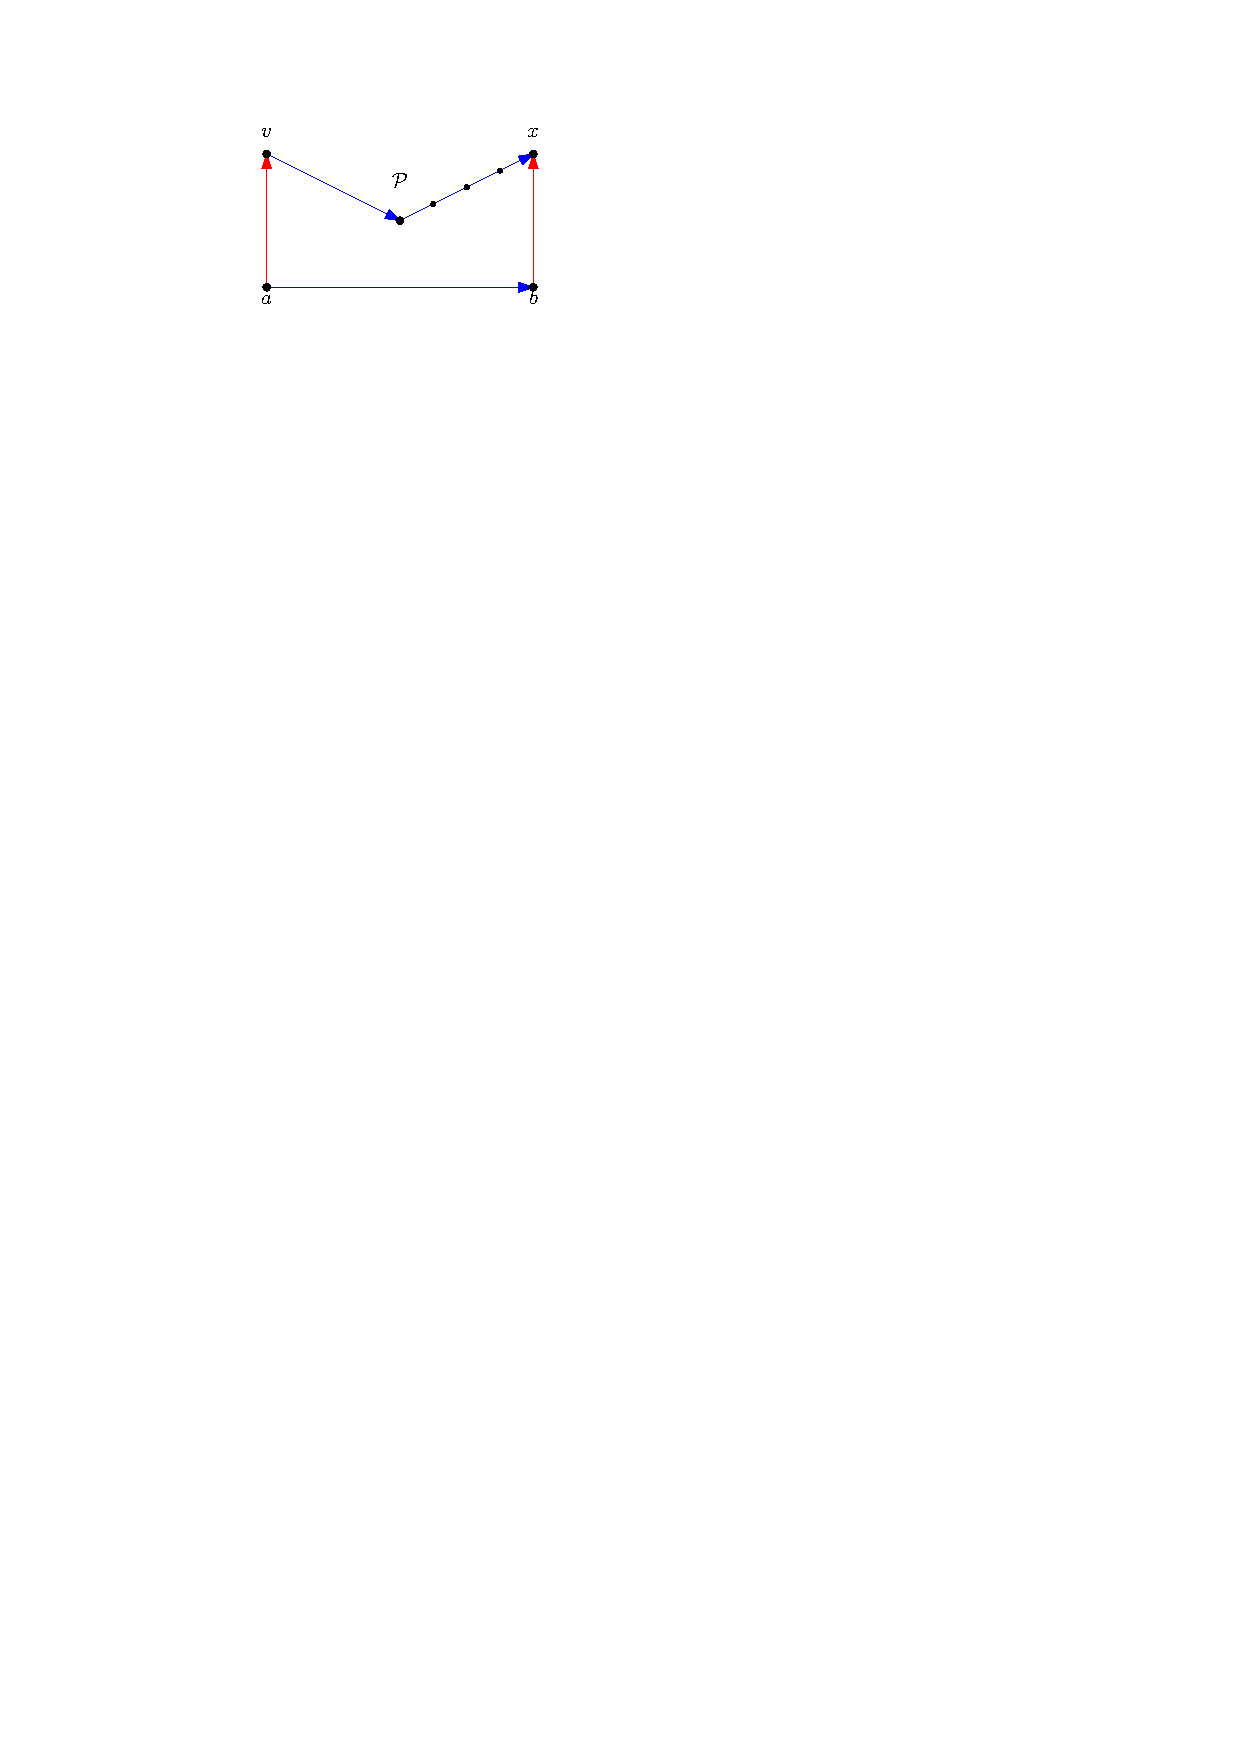
\includegraphics[scale=1]{unifiedAlgo/img/sweep/bottompathChord.pdf}
        \caption{}
        \label{fig:botomPathChord}
      \end{figure}

      The interior of  $vabx \oplus \rev \P$ and has no vertices. Suppose there would be such a vertex then since $\P$ is a bottom path the blue path going trough this vertex has to start at $a$ and end at $b$. But then this gives a blue face with only one edge on its bottom boundary path, hence the interior of this face has no incoming red edges. \fxnote{Or i could make a lemma about face borders somewhere and contradict with that.} So the result is not a \rel. Since our graph is a \rel $vabx \oplus \rev \P$ has no interior vertices.

      This also implies all interior edges are red (by the definition of bottom path) and thus that $ab$ is blue otherwise we would get a monochromatic triangle.

      Now $w$ can not be connected to any vertex in $\P$ that would give a chord. And we do not allow chords in any valid path on the moment we add it. So $w$ can only be connected to $a$ and $b$ and is thus a topfan of size at most $2$. (If it is a topfan at all, since we do not consider topfans of size 1 as topfans.)
    \end{proof}
